\documentclass{beamer}

\title
{SIMT Branch Prediction}
\subtitle{Mitigating Stalls}
\author
{Steven Braeger \and Nick Arnold}
\institute
{
  \inst{1}%
  University of Central Florida
}
\date
{\today}

\begin{document}
\frame{\titlepage}

\begin{frame}
	\frametitle{Generic CPU Core Design}
	\begin{tabular}{c}
		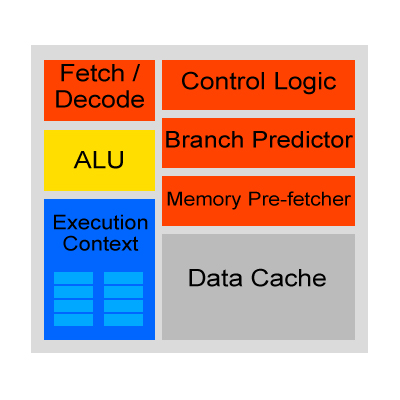
\includegraphics[width=.75\textwidth]{CPU-design.jpg}
	\end{tabular}
\end{frame}

\begin{frame}
	\frametitle{Generic CPU Core Design (cont.)}
	\begin{itemize}
		\item Regular Processor Logic
		\begin{itemize}
			\item Fetch/Decode Logic
			\item ALU for execution
			\item Execution Context (registers, etc.)
		\end{itemize}
		\item Single Thread Speedup Logic
		\begin{itemize}
			\item Control Logic
			\item Branch Predictor
			\item Memory Pre-fetcher
		\end{itemize}
		\item Data Cache
	\end{itemize}
\end{frame}

\begin{frame}
	\frametitle{Generic CPU Core Design (cont.)}
	\begin{itemize}
		\item What does this core do well?
		\begin{itemize}
			\item Single Instruction, Single Data
		\end{itemize}
		\item What does this core do poorly?
		\begin{itemize}
			\item Everything else
		\end{itemize}
	\end{itemize}
\end{frame}

\begin{frame}
	\frametitle{Generic Multicore CPU Core Design}
	\begin{tabular}{c}
		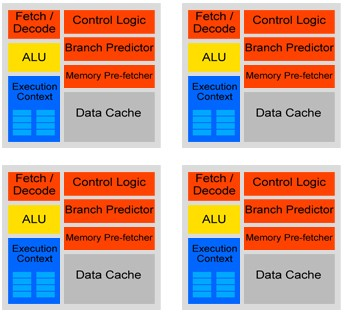
\includegraphics[width=.75\textwidth]{Multicore-CPU-design.jpg}
	\end{tabular}
\end{frame}

\begin{frame}
	\frametitle{Generic Multicore CPU Core Design (cont.)}
	\begin{itemize}
		\item What does this core do well?
		\begin{itemize}
			\item Single Instruction, Single Data
			\begin{itemize}
				\item Either handling multiple independent processes or idling
			\end{itemize}
			\item Multiple Instruction, Single Data
			\begin{itemize}
				\item Fetching independent sequential instructions from one process
			\end{itemize}
		\end{itemize}
		\item What does this core do poorly?
		\begin{itemize}
			\item Anything with multiple data
		\end{itemize}
	\end{itemize}
\end{frame}

\begin{frame}
	\frametitle{Generic GPU Core Design}
	\begin{tabular}{c}
		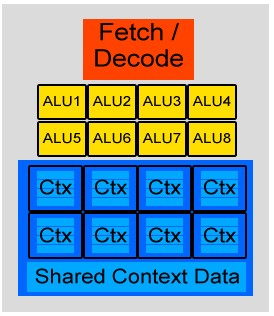
\includegraphics[width=.75\textwidth]{GPU-Design.jpg}
	\end{tabular}
\end{frame}

\begin{frame}
	\frametitle{Generic GPU Core Design (cont.)}
	\begin{itemize}
		\item What's different?
		\begin{itemize}
			\item Removed single threading speedup logic
			\item Removed data cache
			\item Added multiple execution contexts
		\end{itemize}
		\item Why do this?
		\begin{itemize}
			\item GPUs are designed for graphics processing, so they're tailored specifically to those types of instruction streams
			\item Graphics processing exhibits a lot of performing the same operations on many independent data elements
			\item Because of this, multiple instruction streams are not necessary
		\end{itemize}
	\end{itemize}
\end{frame}

\begin{frame}
	\frametitle{Generic GPU Core Design (cont.)}
	\begin{itemize}
		\item What does this core do well?
		\begin{itemize}
			\item Single Instruction, Multiple Data
			\begin{itemize}
				\item Several similar data elements are assigned to a GPU core to perform the same computations on all elements
			\end{itemize}
		\end{itemize}
		\item What does this core do poorly?
		\begin{itemize}
			\item Everything else
		\end{itemize}
	\end{itemize}
\end{frame}

\begin{frame}
	\frametitle{Generic GPU Core Design (cont.)}
	\begin{tabular}{c}
		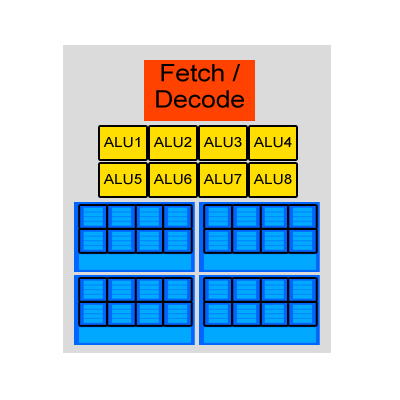
\includegraphics[width=.75\textwidth]{GPU-Design---multiple-contexts.jpg}
	\end{tabular}
\end{frame}

\begin{frame}
	\frametitle{Generic GPU Core Design (cont.)}
	\begin{itemize}
		\item GPUs are able to modify their context storage locations to separate it into various smaller context sizes
		\item This is done to try and hide stalls (more on this later)
		\item All data elements assigned to a GPU core are called a 'warp'
	\end{itemize}
\end{frame}

\begin{frame}
	\frametitle{Generic Multicore GPU Core Design}
	\begin{tabular}{c}
		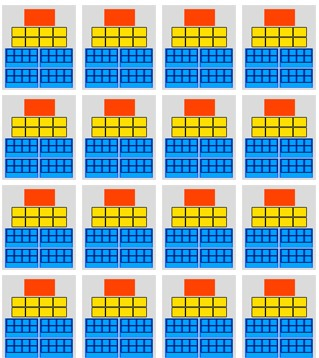
\includegraphics[width=.75\textwidth]{GPU-Design---multiple-cores.jpg}
	\end{tabular}
\end{frame}

\begin{frame}
	\frametitle{Generic Multicore GPU Core Design (cont.)}
	\begin{itemize}
		\item What does this core do well?
		\begin{itemize}
			\item Single Instruction, Multiple Data
			\begin{itemize}
				\item Each core could potentially be assigned the same instruction stream all working on subsets of the dataset
			\end{itemize}
			\item Multiple Instruction, Multiple Data
			\begin{itemize}
				\item GPU has the ability to assign multiple independent tasks, each with its own spatial locality which allows one instruction stream to process multiple data elements
			\end{itemize}
		\end{itemize}
		\item What does this core do poorly?
		\begin{itemize}
			\item Anything with single data
		\end{itemize}
	\end{itemize}
\end{frame}

\begin{frame}
	\frametitle{GPU Context Interleaving}
	\begin{tabular}{c}
		\includegraphics[width=.75\textwidth]{}
	\end{tabular}
	GPU Interleaving image
\end{frame}

\begin{frame}
	\frametitle{GPU Context Interleaving (cont.)}
	\begin{itemize}
		\item By interleaving context execution in this manner, the GPU is always utilizing its ALUs optimally, even though contexts are waiting
		\item However, if the wait time exceeds the number of interleaving contexts, then the GPU must stall
		\item What if we could avoid this?
	\end{itemize}
\end{frame}

\begin{frame}
	\frametitle{Our Proposal}
	\begin{itemize}
		\item Introduce a GPU Branch Predictor with the following features
		\begin{itemize}
			\item Predictor is shared amongst the contexts within a GPU
			\item Predictor table is the size of the instruction stream to avoid collisions
			\item Predictor entries are Smith 2-bit predictors
		\end{itemize}
	\end{itemize}
\end{frame}

\begin{frame}
	\frametitle{Our Proposal (cont.)}
	\begin{tabular}{c}
		\includegraphics[width=.75\textwidth]{}
	\end{tabular}
	Our GPU interleaving replacement image
\end{frame}








\end{document}

